\chapter{Teoretický základ}
\label{2-teorie}

V této kapitole jsou objasněny způsoby monitorování radiační situace,
popsán sběr dat a představen výstupní report.

\section{Ionizující záření}

Ionizující záření je tok buď hmotných částic, nebo fotonů
elektromagnetického záření, které mají schopnost ionizovat atomy
prostředí či excitovat jejich jádra. Příčinou vzniku může být
radioaktivní rozpad, kosmické záření nebo jej lze vytvořit uměle. Je
průvodním jevem jaderných procesů, během nichž se jádro či obal atomu
dostávají do energeticky nestabilního excitovaného stavu. Pro návrat
do stabilního stavu musí vyzářit energii ve formě částic či fotonů
elektromagnetického záření. Podle~způsobu interakce s prostředím se
ionizující záření dělí na dva druhy:

\begin{itemize}
\item \textbf{Přímo ionizující záření} mohou způsobovat jen nabité
  částice, které mají dosta\-tečnou kinetickou energii k vyvolání
  ionizace. Mezi nabité částice patří např. elektrony, částice
  $\alpha$, $\beta$.
	
\item \textbf{Nepřímo ionizující záření} je tvořeno nenabitými
  částicemi (neutrony, fotony), které prostředí přímo sami neionizují,
  ale při vzájemném působení s prostředím předávají svou kinetickou
  energii sekundárním, nabitým částicím, jež následně přímými účinky
  na atomy látku ionizují.
\end{itemize}

% http://astronuklfyzika.cz/JadRadFyzika6.htm
% http://fbmi.sirdik.org/1-kapitola/13/131.html

\subsection{Fyzikální veličiny a jednotky}

\begin{itemize}
\item \textbf{Plošná aktivita}
	
  Množství radioaktivní látky je charakterizováno aktivitou. Jedná se
  o počet radioaktivních přeměn vztažených na jednotku času. Aktivita
  má za jednotku becquerel {[}Bq{]}. U plošných zdrojů záření se
  používá plošná aktivita neboli podíl aktivity a celkové plochy látky
  {[}Bq/m$^2${]}.
	
\item \textbf{Dávkový příkon}
	
  Působení ionizujícího záření popisuje veličina dávka (či také
  absorbovaná dávka), která je určena jako poměr střední energie
  předané ionizujícím zářením látce o~dané hmotnosti. Základní
  jednotkou je gray {[}Gy{]}, který odpovídá energii 1 joule
  absorbované v kilogramu látky. Dávkový příkon je přírůstek dávky v
  časovém intervalu {[}Gy/s{]}. V praxi se používají nižší jednotky
  {[}µGy/h{]} nebo {[}cGy/h{]}.

\item \textbf{Příkon dávkového ekvivalentu}
	
  Na rozdíl od předchozích veličin patří dávkový ekvivalent mezi
  tzv. radiobiologické veličiny, tj. zohledňující účinky působení
  různých druhů záření na živou hmotu. Dávkový ekvivalent je součin
  dávky v uvažovaném bodě tkáně a jakostního činitele, jenž vyjadřuje
  rozdílnou biologickou účinnost různých druhů záření. Příkon
  fotonového dávkového ekvivalentu (\zk{PFDE}) je přírůstek dávkového
  ekvivalentu způsobeného fotony v časovém intervalu
  {[}Sv/s{]}. Prostorový dávkový ekvivalent odpovídá dávkovému
  ekvivalentu, který by uspořádané a rozšířené pole ionizujícího
  záření způsobilo v hloubce d = 10 mm v ICRU kouli\footnote{Koule z
    materiálu adekvátně odpovídajícího tkáni lidského těla o průměru
    30 cm} na rádius vektoru opačného směru, než je orientované
  pole. Příkon prostorového dávkového ekvivalentu (\zk{PPDE}) je
  přírůstek prostorového dávkového ekvivalentu v časovém intervalu
  {[}Sv/s{]}.

% https://www.sujb.cz/aplikace/monras/?lng=cs_CZ#z3
% http://fbmi.sirdik.org/

		\begin{table}[h!]
			\centering
			\caption{Fyzikální veličiny}
			\label{tab:tab_veliciny}
			\begin{tabular}{|c|c|c|}
				\hline
				\textbf{Veličina}           			& \textbf{Jednotka}  & \textbf{Značka}  \\ \hline
				Aktivita								& becquerel			 & {[}Bq{]}			\\ \hline
				Plošná aktivita							& becquerel/m$^2$	 & {[}Bq/m$^2${]}	\\ \hline
				Dávka                      	 			& gray               & {[}Gy{]}         \\ \hline
				Dávkový příkon              			& gray/sekunda		 & {[}Gy/s{]}       \\ \hline
				Dávkový ekvivalent          			& sievert            & {[}Sv{]}         \\ \hline
				Příkon fotonového dávkového ekvivalentu & sievert/sekunda	 & {[}Sv/s{]}       \\ \hline
				Příkon prostorového dávkového ekvivalentu & sievert/sekunda	 & {[}Sv/s{]}       \\ \hline
			\end{tabular}
		\end{table}
\end{itemize}

\section{Monitorování radiační situace}

Pod monitorováním radiační situace je myšleno pravidelné sledování
úrovně ionizujícího záření v okolním prostředí, měření obsahu umělých
radionuklidů ve složkách životního prostředí a potravních řetězců, ale
také sledování radioaktivity v těle člověka. \cite{monras}

Systematické plošné monitorování radiační situace má na území České
republiky počátky v dubnu 1986, kdy došlo k havárii v \zk{JE}
Černobyl. Je zajišťováno pomocí celostátní Radiační monitorovací sítě
(\zk{RMS}) spravované Státním ústavem pro jadernou bezpečnost
(\zk{SÚJB}).

\zk{RMS} běžně operuje v~tzv. normálním režimu, v~případě mimořádné
radiační situace přechází do~tzv. havarijního režimu. Během~normálního
režimu pracují stálé složky \zk{RMS}, jež v první řadě zajišťují
provoz fixních měřících míst a analýzu dat z~nich získaných. 
Mezi~stálé složky \zk{RMS} patří v~první řadě \zk{SÚJB}, Státní ústav
radiační ochrany (\zk{SÚRO}) a Český hydrometeorologický úřad
(\zk{ČHMÚ}). Při~přechodu do~havarijního režimu dochází rovněž 
k~aktivaci pohotovostních složek. Po~zvážení je zahájen radiační
průzkum, který sestává z~dalšího monitorování na~měřících bodech,
pojezdového měření a v~případě potřeby i měření leteckého. \cite{suro}
Všechny získané informace jsou potřebné pro~rozhodování o~opatřeních
vedoucích ke~snížení nebo odvrácení ozáření.

% (1) http://www.mocr.army.cz/informacni-servis/zpravodajstvi/chemici-se-specialisty-statniho-ustavu-radiacni-ochrany-spolecne-monitorovali-radiaci-z-vrtulniku-118918/

% (2) https://www.suro.cz/cz/rms	

\subsection{Sběr dat}	

Mezi hlavní způsoby monitorování radiační situace patří:

\begin{itemize}
\item \textbf{napevno umístěné detektory (měřící body)}
	
\begin{figure}[H]
    \centering
      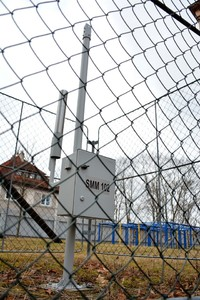
\includegraphics[width=150pt]{./pictures/03_merici-sonda-v-libereckych-kasarnach_2.jpg}
      \caption[Měřící sonda libereckých chemiků]{Měřící sonda libereckých chemiků
      (autor: \href{http://www.acr.army.cz/informacni-servis/zpravodajstvi/armadni-radiacni-monitorovaci-site-nacvicoval-zasah-pri-radiaci-131355/}{kapitán Ing. Jakub Šimíček})}
      \label{fig:sonda}
\end{figure}
	
Jedním ze způsobů hodnocení radiační situace je zjištění odchylek od
dlouhodobého průměru \zk{PFDE}, resp. \zk{PPDE}. Dlouhodobě měřené
hodnoty \zk{PFDE} na území České republiky se pohybují mezi 0,1 až 0,2
{[}µSv/h{]}\footnote{Zdroj:
  \url{https://www.sujb.cz/aplikace/monras/}}. Tato měření jsou nepřetržitě
prováděna na pevně umístěných detektorech.
	
Základním systémem, umožňujícím průběžné sledování radiační situace na
území ČR, je Síť včasného zjištění (\zk{SVZ}) spravovaná Regionálními
centry (RC) \zk{SÚJB}, \zk{SÚRO}, \zk{ČHMÚ} a Armádou ČR. SVZ je v
okolí a uvnitř areálu jaderných elektráren Dukovany a Temelín doplněna
teledozimetrickými systémy (\zk{TDS}), jejichž činnost je zajišťována
ČEZ, a.s. Detekční jednotky \zk{SVZ} i \zk{TDS} obsahují dva detektory
s různým rozsahem měření veličiny \zk{PFDE}. Dalším způsobem zjištění
odchylek od průměru jsou integrální měření fotonových,
resp. prostorových dávkových ekvivalentů zjišťovaná v měřících místech
s integrálními dozimetry, které tvoří teritoriální síť a lokální síť v
okolí \zk{JE}.
	
		
\item \textbf{pozemní monitorování}
	
\begin{figure}[H]
    \centering
      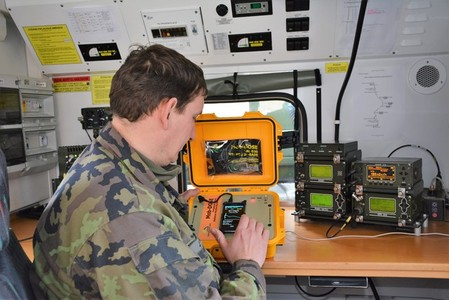
\includegraphics[width=250pt]{./pictures/02_mereni-radiace-v-terenu-z-vozidla_2.jpg}
      \caption[Liberecký chemik měří radiaci v terénu ve speciálním vozidle]{Liberecký chemik měří radiaci v terénu ve speciálním vozidle
      (autor: \href{http://www.acr.army.cz/informacni-servis/zpravodajstvi/armadni-radiacni-monitorovaci-site-nacvicoval-zasah-pri-radiaci-131355/}{kapitán Ing. Jakub Šimíček})}
      \label{fig:pozemni}
\end{figure}
	
Sběr dat při pojezdovém měření je prováděn z vozidla jedoucího
rychlostí 40 km/h po určené trase. Spolu s měřenou hodnotou se
zaznamenává čas a poloha měření.
	
Při naměření předem stanoveného dávkového příkonu osádka vozu již dále
nepokra\-čuje ve směru rostoucích hodnot do epicentra
výbuchu. \uv{Takováto úroveň se pouze vytyčí a souřadnice jejího
  naměření se zahlásí radiostanicí na sběrné stanoviště (veliteli
  jednotky radiačního průzkumu, popřípadě na analytickou skupinu),}
popi\-suje nadporučík Jiří Komárek, starší důstojník Skupiny
monitorování a leteckého průzkumu 314. centra výstrahy
\zk{ZHN}. Následně se osádka vrací zpět po stejné trase.
	
Právě závislost pozemního průzkumu na trasách přesunu, tj. cestách, a
vystavení osádky vyšším hodnotám ionizujícího záření je jeho největší
nevýhodou. Proto se provádí jako doplněk k měření leteckému. Hlavním
zdrojem informací se stává ve~chvíli, kdy povětrnostní podmínky
nedovolí realizovat letecké monitorování.
	
Pozemní monitorování zajišťují \zk{SÚJB}, \zk{SÚRO}, Hasičský
záchranný sbor ČR, Gene\-rální ředitelství cel, Armáda ČR, Policie ČR a
ČEZ, a.s.
	
\item \textbf{letecké monitorování}
	
  Letecké monitorování je prováděno z vrtulníku letícího ve výšce asi
  100 m nad~teré\-nem po předem určených trasách. Naměřené údaje jsou
  přepočítány na úroveň radiace ve výšce 1 m nad terénem. Oproti
  pojezdovému měření si letecký průzkum může dovolit prozkoumat
  kontaminovaný prostor více do hloubky. Úkolem specialistů na palubě
  však je sledování měřených dávkových příkonů, aby eventuálně mohli
  buď upravit parametry průzkumu (rychlost, výška letu), nebo změnit
  trasu letu. Cílem je rychlé, orientační zmapování velké oblasti bez
  ohledu na~charakter terénu.
	
  \uv{V případě jaderného výbuchu by mohl být letecký průzkum
    potenciálně využit ke~zmapování radioaktivní stopy, kterou takový
    výbuch po vypadání částic zanechá. Důležité jsou tady samozřejmě
    vhodně zvolené podmínky průzkumu,} doplňuje dále nadporučík
  Komárek.
	
  Omezujícími podmínkami leteckého průzkumu je povětrnostní situace a
  doba, po kterou je třeba vyčkat, než vypadají radioaktivní částice
  na zemský povrch. Během čekání lze předběžně určit orientační
  dávkové příkony v epicentru vztažené na odhad mohutnosti výbuchu, na
  jejichž základě se rozhodne o provedení průzkumu ve vhodném časovém
  horizontu (po \uv{vymření} krátkodobých radionuklidů, kdy radiace v
  epicentru poklesne). Následně lze provést průzkum v souladu s
  principem \zk{ALARA}, tedy že dávka ionizujícího záření, které je
  osoba vystavena, má být tak nízká, jaké lze rozumně dosáhnout.
	
  Letecké monitorování v ČR provádí \zk{SÚRO} a Armáda ČR.

\end{itemize}
	
Nově získané hodnoty radiačního monitorování jsou při vkládání do
programu \zk{MonRaS} porovnávány s informačními úrovněmi. Informační
%%% ML: v jedne vete 2x "prekroceni", prosim opravit
úrovně existují dvě: 1. a 2. IU. Při jejich překročení jsou zjišťovány
důvody přesáhnutí a případně provedeny kroky nutné k odstranění
příčiny.
	
\subsection{Armádní radiační monitorovací síť}	
	
% zdroj: JK
% http://www.vvubrno.cz/userstorage/files/pdf/prospekty/svz-arms-sit-vcasneho-zjisteni.pdf
% http://www.acr.army.cz/informacni-servis/zpravodajstvi/armadni-radiacni-monitorovaci-site-nacvicoval-zasah-pri-radiaci-131355/
	
U Armády České republiky se monitorováním radiační situace zabývají
dvě jednotky.
	 
314. centrum výstrahy proti zbraním hromadného ničení (\zk{ZHN}) v
Hostivici je zodpovědné především za letecký radiační průzkum a
monitorování radiační situace pomocí Sítě včasného zjištění patřící do
Armádní radiační monitorovací sítě (\zk{SVZ ARMS}). Jedná se o
soustavu 16 stacionárních sond (původně jich bylo 17, ale sonda v
Rakovníku byla zrušena a dosud nebyla nahrazena). \zk{AČR} svými daty
ze~\zk{SVZ ARMS} přispívá do celostátní \zk{RMS}, kterou spravuje
\zk{SÚJB}.
	 
K provedení leteckého radiačního průzkumu AČR využívá vrtulník 
Mil~Mi-17. V~současné době AČR disponuje gama spektrometrickým systémem
IRIS (Integrated Radiation Information System), přístrojem MobDOSE a
palubním detektorem~DP-3a. IRIS umí měřit nejen dávkový příkon a
dávku, ale především energetické spektrum detekovaného záření gama,
tj. lze jej využít ke gama spektrometrii.
	
Za pozemní průzkum jsou zodpovědné především jednotky 31. pluku
radiační, chemické a biologické ochrany v Liberci. Sběr dat při
pojezdovém měření je prováděn z vozidla Land Rover LR-110, lehkého
obrněného kolového transportéru BRDM-2 nebo džípu UAZ-469 (postupně
vyřazován). Přístroje používané k měření dávkového příkonu jsou DP-98,
AS-67 nebo DP-3b a jsou pevně spojené s vozidlem.
	 
	 
\section{Textový report}
% JK
% https://systematic.com/defence/products/a/military-messaging/app-11-and-adatp-3/	

APP-11 je katalog, který specifikuje formát textových zpráv (\zk{MTF})
používaných v \zk{NATO} ke komunikaci se spřátelenými silami. Poslední
verze katalogu APP-11 obsahuje více než 400 zpráv pokrývajících každý
aspekt operací NATO, při němž se vyskytuje potřeba předávání informací
pomocí standardizovaných zpráv. Zprávy jsou sestaveny na základně
pravidel uvedených v technické publikaci ADatP-3.

\zk{MTF} zprávy se skládají ze dvou částí - hlavičky a těla. Hlavička
zahrnuje data o~původci, příjemci či klasifikaci. Tělo pak obsahuje
předávanou informaci ve formátu specifikovaném v APP-11.

\begin{figure}[H]
    \centering
      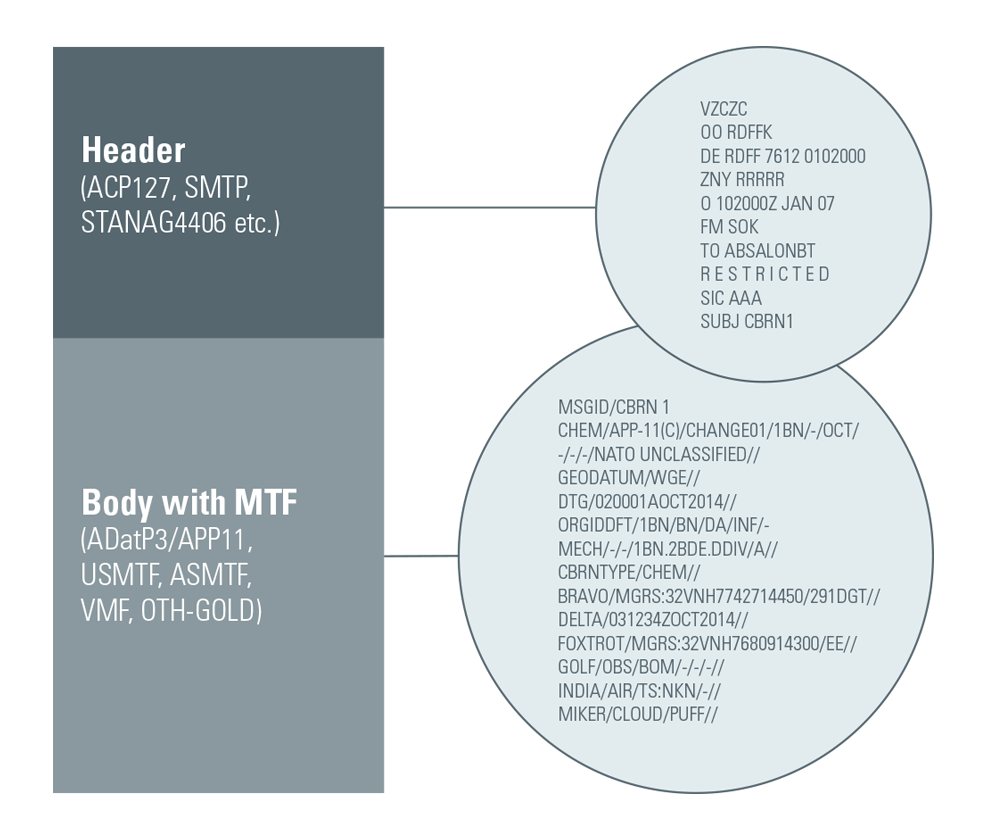
\includegraphics[width=350pt]{./pictures/Military-Messaging-white-borders-988px.png}
      \caption[Struktura zprávy MTF]{Struktura zprávy MTF
      (zdroj: \href{https://systematic.com/defence/products/a/military-messaging/app-11-and-adatp-3/}{SYSTEMATIC})}
      \label{fig:systematic}
  \end{figure}
  
Hlavní výhody \zk{MTF} zprávy:

%%% ML: tucne pismo pro cely vycet je mozna az prilis
\begin{itemize}
	\item{jasně strukturovaný obsah je pochopitelný a předchází nedorozuměním}
	\item{je přenositelná mezi různými národy a systémy}
	\item{při přenosu požaduje malou šířku vlnového pásma}
	\item{je vhodná pro strojové zpracování}
\end{itemize}

Výstupem ze zásuvného modulu je textový report ve formátu v souladu s
katalogem APP-11 (viz kapitola \ref{output}). Jedná se o seznam 
souřadnic lomových bodů polygonů v systému \zk{MGRS}, který bude 
součástí \zk{MTF} zprávy.

\subsection{Military grid reference system}

Hlásný systém \zk{MGRS} je systém udávání polohy používaný
Severoatlantickou aliancí (\zk{NATO}). Využívá Mercatorovo příčné
válcové konformní zobrazení (\zk{UTM}), případně \zk{UPS}.

Na rozdíl od jiných souřadnicových systémů, které vyjadřují polohu
pomocí dvojice hodnot (šířka/délka, x/y), MGRS využívá jen jednu
hodnotu a to alfanumerický řetězec znaků. Ten je tvořen třemi údaji:

\begin{itemize}
	\item \textbf{označení zóny}
	
          Jedna zóna je tvořena sférickým čtyřúhelníkem referenčního
          elipsoidu, jenž je vymezen zeměpisnými poledníky a
          rovnoběžkami. Sférické čtyřúhelníky vznikají rozdělením
          povrchu Země do 60 poledníkových zón o šířce 6°, které jsou
          následně děleny ve směru rovnoběžek na 19 vrstev po 8° a 1
          vrstvu o výšce 12°.
	
          Poledníkové pásy jsou číslovány od 1 do 60 od obrazu
          poledníku 180° z. d. směrem na východ. Vrstvy jsou značeny
          velkými písmeny latinské abecedy C-X (s vynecháním písmen I
          a O vzhledem k jejich podobnosti s číslicemi) od obrazu
          rovnoběžky 80° j. š. na sever.
	
          Jedinečné označení zóny je složeno z čísla poledníkového
          pásu následovaného písmenem rovnoběžkového pásu (např. 33U).
	
	\item \textbf{označení čtverce 100 x 100 km}
	
          Jednotlivé zóny jsou rozděleny na čtverce o hraně 100 km
          sítí čar rovnoběžných s obrazem příslušného osového
          poledníku a rovníku. Jelikož se poledníkové pásy směrem k
          pólům zužují, zóny obsahují určitý počet úplných čtverců a
          na krajích neúplné čtverce o proměnlivé šířce.
	
          Pro označení sloupců jsou použita písmena A-Z (s vynecháním
          I a O), značení začíná u obrazu poledníku 180° z. d. a
          pokračuje směrem na východ, po písmenu Z se celá řada opět
          opakuje. Vrstvám jsou přidělena písmena A-V (bez I a
          O). První vrstva lichých poledníkových pásů je značena
          písmenem A, u sudých pásů začíná písmenem F. Po písmenu V se
          abeceda opakuje.
	
          Označení čtverce se skládá ze dvou písmen - označení sloupce
          a vrstvy (např. VR)
		
	\item \textbf{souřadnice bodu ve 100 km čtverci}
	
          V rámci čtverce je upřesněna poloha bodu za pomoci n+n
          číslic, kde první sada číslic určuje východní souřadnici od
          levého kraje čtverce a druhá sada severní souřadnici od
          okraje spodního. Podle přesnosti vyjádření polohy bodu n
          nabývá hodnot 1, 2, 3, 4 nebo 5.
	
		\begin{itemize}
				\item 1+1 číslice pro souřadnici s přesností 10 km (\textit{54})
				\item 2+2 číslice pro souřadnici s přesností 1 km (\textit{5748})
				\item 3+3 číslice pro souřadnici s přesností 100 m (\textit{577484})
				\item 4+4 číslice pro souřadnici s přesností 10 m (\textit{57704840})
				\item 5+5 číslic pro souřadnici s přesností 1 m (\textit{5770048400})
		\end{itemize}	
		 
\end{itemize}

\begin{figure}[H]
    \centering
      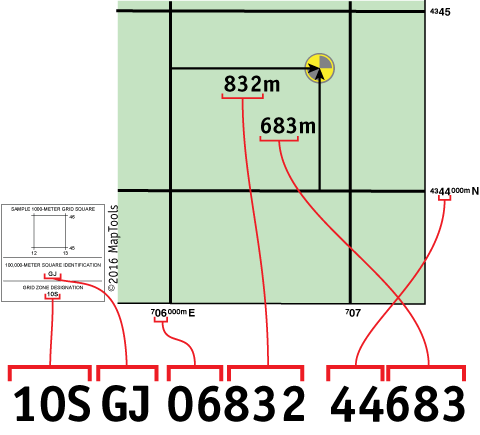
\includegraphics[width=250pt]{./pictures/MGRS_tvorba.png}
      \caption[Postup tvorby souřadnic MGRS]{Postup tvorby souřadnic MGRS
      (zdroj: \href{https://www.maptools.com/tutorials/mgrs/quick_guide}{MapTools})}
      \label{fig:maptools}
\end{figure}
  
Poloha Fakulty stavební ČVUT v Praze by tedy pomocí hlásného systému
%%% ML: doplnit...
MGRS s přesností na metry byla vyjádřena řetězcem 33UVR5623950375.

Standardem NATO je rozlišení 10 m \cite{wiki}, Armáda ČR pro výstup
zásuvného modulu požaduje přesnost na 1 m.

Východní a severní souřadnice v systému MGRS se vždy vztahují k levému
dolnímu rohu čtverce. Při přechodu na nižší přesnost se souřadnice
nezaokrouhlují, ale přebytečné číslice se odříznou, aby bylo
zajištěno, že bod zůstane ve správném čtverci s nižší přesností.

% zdroje: https://www.vugtk.cz/slovnik/5479_hlasny-system-mgrs -
% základní definice
% http://uhulag.mendelu.cz/files/pagesdata/cz/geodezie/geodezie1/souradnicove_systemy.pdf
% (str. 48) http://www.diverzanti.cz/cl_36a - nejvíc
% https://en.wikipedia.org/wiki/Military_Grid_Reference_System
